\section{MANAGEMENT NAPÁJECÍHO NAPĚTÍ INTEGROVANÉHO OBVODU}
UVLO (řízení obvodu pomocí vstupního napájecího napětí, komparace vstupního napětí), Power on Reset (UV signál), realizace a výpočet nastaveni komparačních úrovní

\begin{figure}[h]
   \begin{center}
     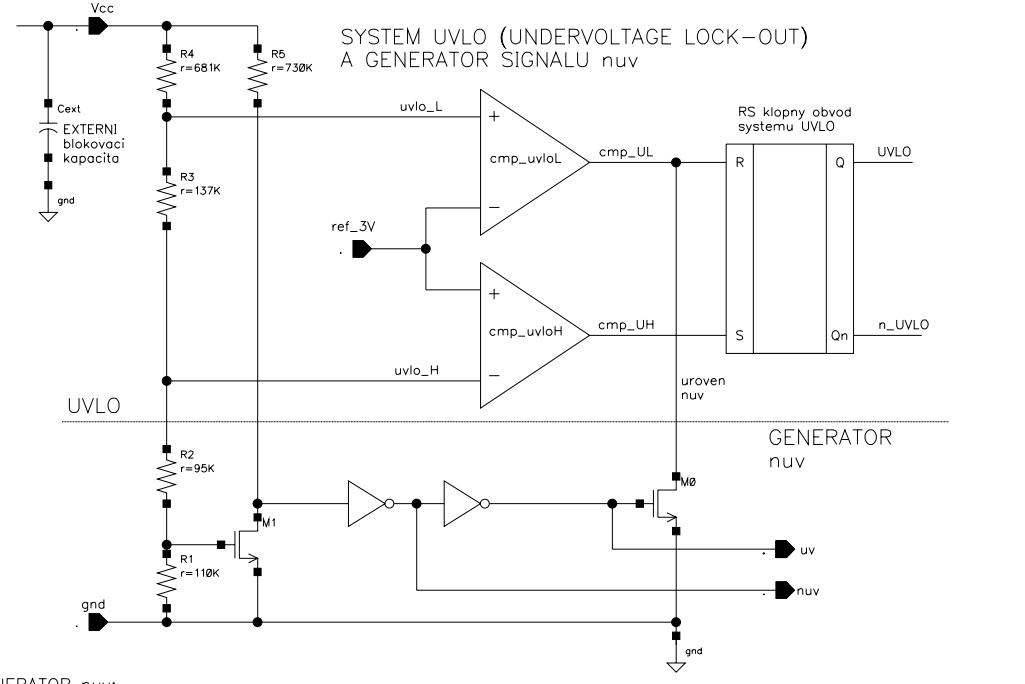
\includegraphics[scale=0.5]{images/UVLO.png}
   \end{center}
   \caption{Systém UVLO}
\end{figure}

\subsection{UVLO}
UVLO systém se aktivuje, pokud napájecí napětí Ucc dosáhne "zespodu" hodnoty UccH a zablokuje (disable) IO pokud napětí poklesne pod UccL. Po zapnutí se na Ucc pinu objeví lenárně rostoucí napětí. Na začátku je hodnota uvloL i uvloH nižší než 3 V, což způsobí, že výstup komparátoru cmpUVLOL je v úrovni L a výstup komparátoru cmpUVLOH je v úrovni H. Nízká úroveň compUVLOL na výstupu vyresetuje RS klopný obvod, na jeho Q výstupu se objeví nízká úroveň, která blokuje IO. Napětí Ucc pak dosáhne takové úrovně, že je vyšší, než komparační napětí 3 V, což způsobí přechod komparátoru compUVLOL do stavu H.

Napětí na vstupu uvloH je zatím nižší než 3 V, na výstupu komparátoru compUVLOH je stále úroveň H a funkce IO je blokovaná. Pokud hodnota Ucc dosáhne takové úrovně UccH, že napětí na vstupu uvloH přesáhne úroveň 3 V, přejde vstup komparátoru cmpUVLOH do úrovně L a změní se stav RS obvodu, na výstupu Q se objeví stav High, což odblokuje IO.

Pokud napětí Ucc klesne pod úroveň UccH, přejde Q klopného RS obvodu do H, ale RS obvod si stále pamatuje svůj předchozí stav a IO není blokován. 

Pokud napětí Ucc klesne pod UccL, přejde výstup komparátoru cmpUVLOL do stavu L, což změní stav klopného RS obvodu a na výstupu Q se objeví stav L a IO je tak blokován. 

Úrovně UccH a UccL se vypočítají následovně:

\begin{equation}
Ucc_{H} = U_{ref}*\frac{R_{1}+R_{2}+R_{3}+R_{4}}{R_{1}+R_{2}}
\end{equation}

\begin{equation}
Ucc_{L} = U_{ref}*\frac{R_{1}+R_{2}+R_{3}+R_{4}}{R_{1}+R_{2}+R_{3}}
\end{equation}

\subsection{Signál UV}
Signál UV slouží k nastavení vnitřní logiky celého systému při zapnutí napájecího napětí. Předpokládá se, že napájecí napětí je blokováno kondenzátorem, takže náběh napětí Ucc je poměrně pomalé. Při zapnutí narůstá na pinu Ucc napětí. Pokud je jeho hodnota nízká, tak NMOS M1 je zavřený a na jeho drainu je úrověň H a signál NUV je na úrovni L.

Nízkou úroní signálu NUV se nastaví (resetuje) logika celého IO. Signál NUV přejde do úrovně H a okamžiku, kdy napětí na pinu Ucc dosáhne takové úrovně, že tranzistor M1 sepne z H do L (signál NUV z L do H) je určena prahová hodnota napětí Ugs = Ugsr tranzistoru M1, při níž M1 sepne dělič R1 až R4.

Prahová hodnota Ugs je asi Ugsr = 0,85 V. Z tohoto se určí hodnota Uccr při níž signál NUV přechází z L do H.

\begin{equation}
U_{ccr} = U_{gsr}*\frac{R_{1}+R_{2}+R_{3}+R_{4}}{R_{1}}
\end{equation}
